\section{The TOV equation}

We will model a star as being made up of a \emph{perfect fulid}, with energy density $u$ and pressure $p$.
The relationship between the pressure and energy density of a substance is called the \emph{equation of state}, or EOS, and has the form
\begin{equation}
    \label{EOS}
    f(p, u, \{\xi_i\}) = 0,
\end{equation}
where $\{\xi_i\}$ are possible other thermodynamic variables.
We will be working at zero temperature, in which case there are no other free thermodynamic variables.
This allows us to, at least locally, express the energy density as a function ofthe pressure, $u = u(p)$.
The stress-energy tensor of a perfect fluid is\todo{Forklar}
%
\begin{equation}
    T_{\mu \nu} = (u + p) u_\mu u_\nu - p g_{\mu \nu},
\end{equation} 
where $u_\mu$ is the 4-velocity of the fluid.
In the rest frame of the fluid, we may write 
\begin{equation}
    v_\mu = \left(v_0, 0, 0, 0\right).
\end{equation}
This, together with the normalization condition of 4-velocities, $v_\mu v^\mu = 1$, allows us to calculate that
%
\begin{equation}
    v_\mu v^\mu = g^{\mu \nu} v_\mu v_\nu = g^{00} (v_0)^2 = 1.
\end{equation}
%
Using \autoref{spherically symmetric metric}, we see that
\begin{equation}
    v_0 = e^{\alpha(r)}.
\end{equation}
%
This gives us the stress-energy tensor of the perfect fluid in its rest frame,
%
\begin{equation}
    T_{\mu \nu} 
    =
    \left(
        \begin{matrix}
            u{\left(r \right)} e^{2 \alpha{\left(r \right)}} & 0 & 0 & 0\\0 & 
            p{\left(r \right)} e^{2 \beta{\left(r \right)}} & 0 & 0\\
            0 & 0 & p{\left(r \right)} r^{2} & 0\\
            0 & 0 & 0 & p{\left(r \right)} r^{2} \sin^{2}{\left(\theta \right)}
        \end{matrix}
    \right).
\end{equation}
%
We will use the $tt$ and $rr$ components of the Einstein field equations, which are
%
\begin{align}
    \label{tt equation}
    8 \pi G r^{2} u{\left(r \right)} e^{2 \beta{\left(r \right)}} 
    & =   2 r \frac{d}{d r} \beta{\left(r \right)} + e^{2 \beta{\left(r \right)}} - 1 \\
    \label{rr equation}
    8 \pi G r^{2} p{\left(r \right)} e^{2 \beta{\left(r \right)}} 
    & = 2 r \frac{d}{d r} \alpha{\left(r \right)} - e^{2 \beta{\left(r \right)}} + 1.
\end{align}
%
In analogy with the Schwartzhild metmric, we define the function $m(r)$ by
\begin{equation}
    e^{2 \beta(r)} = \left(1 - \frac{2 G m(r)}{r} \right)^{-1}. 
\end{equation}
Substituting this into \autoref{tt equation} yields 
\begin{equation}
    \label{diff eq mass}
    \diff{m(r)}{r} = 4 \pi r^2 \, u(r).
\end{equation}
The solution is simply
\begin{equation}
    \label{mass relation}
    m(r) = 4 \pi \int_0^r \dd r' \, {r'}^2 u(r').
\end{equation}
We see that $m(r)$ is the matter content contained within a radius $r$.
If $u = 0$ for $r > R$ and $m(r>R) = M$, then the metric on a constant-time surface, i.e. $\dd t = 0$, is
%
\begin{equation}
    \dd s^2
    = 
    \left( 1 - \frac{2 G M}{r^2} \right)^{-1} \dd r^2 
    + r^2 (\dd \theta^2 + \sin^2 \theta \, \dd\varphi^2).
\end{equation} 
%
This is the same as for the Schwarzschild solution.

Using the Bianchi identity, \autoref{Einstein tensor bianchi identity}, together with EInstein's equation, we find that
%
\begin{equation}
    \nabla^\mu G_{\mu \nu} = \nabla^\mu T_{\mu \nu} = 0.
\end{equation}
%
The $r$-component of this equation is
%
\begin{equation}
    \nabla_\mu T^{\mu r} 
    =
    \partial_r T^{rr} 
    + \Gamma^\mu_{\mu \nu} T^{\nu r} 
    + \Gamma^r_{\mu \nu} T^{\mu \nu},
\end{equation}
%
where we have used the particular form of $T_{\mu \nu}$ and the Christoffel symbols to eliminate vanishing terms.
We calculate
%
\begin{align*}
    \nabla_\mu T^{\mu r} 
    & = 
    \partial_r \left(p e^{-2\beta}\right)
    + (2 \Gamma^r_{rr} + \Gamma^t_{tr}) T^{rr} 
    + \Gamma^r_{tt}T^{tt} \\ 
    &=   e^{-2\beta} \left( \partial_r p + p \partial_r \alpha + u \partial_r \alpha \right) = 0.
\end{align*} 
%
This allows us to relate $\alpha$ to $p$ and $u$, via
\begin{equation}
    \partial_r \alpha = - \frac{\partial_r p}{p + u}
\end{equation}
%
When we substitute this, together with the definition of $m(r)$, into \autoref{rr equation}, we obtain
%
\begin{equation}
    \label{TOV}
    \diff{p}{r}
    =
    -
    \frac{G}{r^2} 
    \left(4 \pi r^{3} p + m \right) 
    \left(u + p \right)
    \left(1 - \frac{2 G m}{r}\right)^{-1},
\end{equation}
%


the Tolman-Oppenheimer-Volkoff (TOV) equation.
\todo{Ref originale publikasjon}
To summarize, we have three unknown functions, $u(r)$, $p(r)$, and $m(r)$.
The equation of state, \autoref{EOS}, determine $u = u(p)$, eliminating one unknown.
The two differential equations \autoref{mass relation} and \autoref{TOV}, together with inital conditions such as $p(0) = p_0$ and $m(0) = 0$, then yield $p(r)$ and $m(r)$ when integratied.

We define dimensionless varaibles and characteristic dimensions,
%
\begin{equation}
    u = u_0 \tilde u, \, p = u_0 \tilde p, \, m =  m_0 \tilde m, r = r_0 \tilde r.
\end{equation}
%
Here, quantities with subscript $0$ are dimensionfull constants, the characteristic dimensions, while the tilde indicates a dimensionless variable.
Inserting this into \autoref{diff eq mass} and \autoref{TOV} yields
%
\begin{align}
    \label{mass relation dimensionless}
    \diff{ \tilde m}{\tilde r} & = 3 k_2 \tilde r^2 \tilde u \\
    \label{TOV dimensionless}
    \diff{\tilde p}{\tilde r} & 
    = - \frac{k_1}{\tilde r^2} \left(\tilde p + \tilde u\right) \left(3 k_2 \tilde r^3 \tilde p + \tilde m\right) 
    \left(1 - \frac{2 k_1  \tilde m}{\tilde r}\right)^{-1},
\end{align}
%
where we have defined the dimensionless groups
%
\begin{equation}
    \label{dimensionless groups}
    k_1 = G \frac{m_0}{r_0}, \quad k_2 =  \frac{4 \pi}{3} \frac{r_0^3 u_0}{m_0}.
\end{equation}
%


\subsection*{Incompressible fluid}

The simplest model for a fluid is an incompressible fluid, where the energy density is independent of the pressure.
In this case, the energy density of the star will be constant for a radius $r < r_0$, before it drops to zero,
%
\begin{equation}
    u(r) = u_0 \, \theta (r_0 - r),
\end{equation}
%
where $u_0$ is a constant and $\theta(x)$ the Heaviside step funciton.
We have chosen the radius to be the characteristic dimension $r_0$.
Inserting this into the differential equation of the mass function, \autoref{mass relation dimensionless}, yields
%
\begin{equation}
    \tilde m(\tilde r) = k_2 \tilde r^3,
\end{equation}
%
when $r < r_0$.
For $r \geq r_0$, or $\tilde r \geq 1$, this relationship is simply constant $\tilde m(\tilde r) = \tilde m(1) = k_2$.
We choose $m_0$ to be the gravitational mass of the star, i.e. $m_0 = \frac{4 \pi }{3} r_0^3 u_0$, which is equivalent to setting $k_2 = 1$.
With this the TOV equation, \autoref{TOV dimensionless}, becomes
%
\begin{equation} 
    \diff{\tilde p}{\tilde r} = - k_1 r \frac{(1 + p)(1 + 3 p)}{(1 - 2 k_1 r^2)}.
\end{equation}
%
This is a separable ODE, and each variable may be integrated separately.
Using
%
\begin{align}
    \int \frac{\dd p}{(1 + p)(1 + 3p)} 
    & = \frac{1}{2} \ln \frac{3p + 1}{p + 1} + \const , \\
    \int \frac{\dd r \, r}{(1 - 2 r^2)} 
    & = \frac{1}{4}\ln\left(1 - 2 r^2 \right)
    + \const,
\end{align}
%

together with the boundary condition $p(r = r_0) = 0$, we get 
%
\begin{equation}
    \label{pressure afo r incompressible}
    \tilde p(\tilde r) 
    = 
    - \frac{\sqrt{1 - 2 k_1} - \sqrt{1 - 2 k_1 \tilde r^2}}{3 \sqrt{1 - 2 k_1 } - \sqrt{1 - 2 k_1 \tilde r^2}}.
\end{equation}
%
We see that the star is wholly characterized by $k_1$.
In \autoref{fig: pressure incompressible fluid}, we have plotted the pressure as a function of radius for some values of $k_1$.
As $k_1$ approaches $0.\bar 4 = 4/9$, the pressure at the center of the star start to increas rapidly.
From the denominator of \autoref{pressure afo r incompressible} at $r\rightarrow 0$, we can set the limit
%
\begin{equation}
    k_1 = G \frac{m_0}{r_0} \leq \frac{4}{9}.
\end{equation}
%
This is an absolute limit of the mass of an object given its radius or vice versa.
General relativity does not allow for a static solution with energy densities greater than this; any such configuration would collapse in on itself~\autocite{carrollSpacetimeGeometryIntroduction2019}.

\begin{figure}
    \centering
    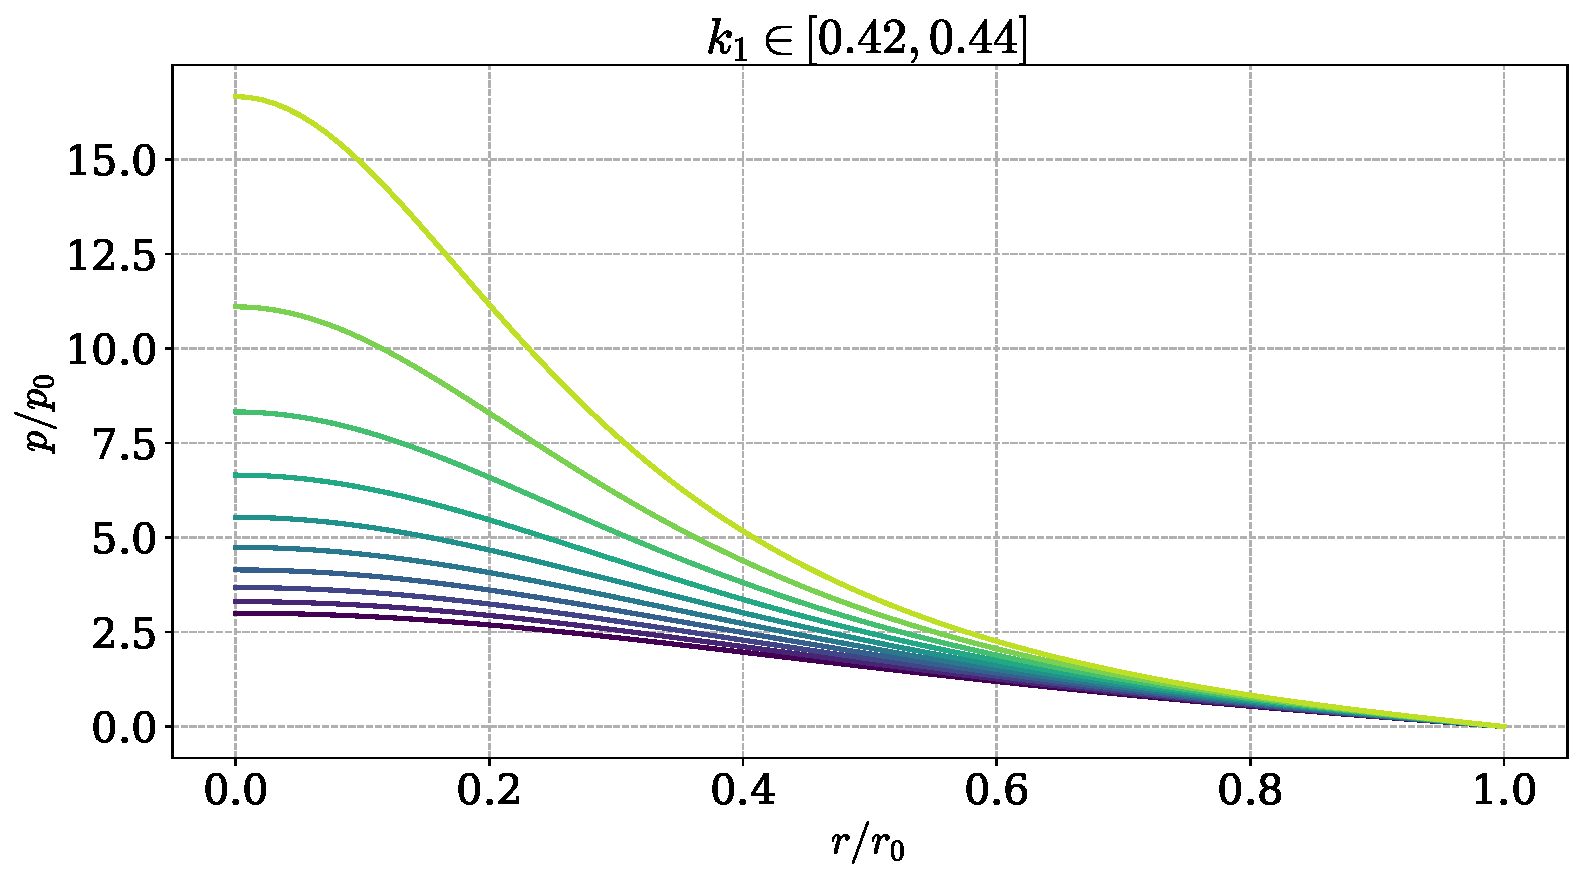
\includegraphics[width=0.8\textwidth]{figurer/scripts/incompressible.pdf}
    \caption{The pressure of a star made up of a incompressible fluid, as a funciton of its radius. The different lines corresponds to different total masses.}
    \label{fig: pressure incompressible fluid}
\end{figure}


\subsection*{Free fermi gas}

A non-interacting free Fermi gas is governed by the Lagrangian
\todo{Skrive om thermal field theory}
%
\begin{equation}
    \Ell = \bar \psi (i \slashed \partial - m) \psi.
\end{equation}
%
This gas has the free energy density, after dropping an infinite constant, 
%
\begin{equation}
    \Eff = \frac{2}{\beta}\int \frac{\dd^3 p}{(2 \pi)^3} \left[
        \ln(1 + e^{-\beta(\omega - \mu)})
        + 
        \ln(1 + e^{-\beta(\omega + \mu)})
    \right],
\end{equation}
%
where $\omega = \sqrt{p^2 + m^2}$.
The free energy density is related to the thermodynamic variables at interest by
%
\begin{equation}
    p = - \Eff, \quad n = - \diffp{\Eff}{\mu}, \quad u = \Eff + \mu n.
\end{equation}
%
We may write the free energy density, and thus the pressure, in terms of the Fermi distribution $n_f$, by integrating by parts, leaving
%
\begin{equation}
    P = \frac{2}{3}\int \frac{\dd^3 p}{(2 \pi)^3} 
    \frac{p^4}{\omega}
    [n_f(\omega - \mu) + n_f(\omega + \mu)],
\end{equation}
%
where we have used 
%
\begin{equation}
    \int_0^\infty \dd p \, p^2 \ln\left[1 + e^{-\beta(\omega \pm m)}\right]
    = 
    \frac{1}{3} p^3\ln\left[1 + e^{-\beta(\omega \pm m)}\right] \bigg |_0^\infty
    + \frac{1}{3} \int_0^\infty \dd p \, \frac{ \beta p^4}{\omega}n_f(\omega \pm \mu).
\end{equation}
%
The particle density $n$ is
%
\begin{equation}
    n = 2 \int \frac{\dd^3 p}{(2 \pi)^3}
    \left[
        n_f(\omega + \mu)
        -
        n_f(\omega - \mu)
    \right].
\end{equation}
%
This gives us a energy density
%
\begin{equation}
    u
    =
    -\frac{1}{\pi^2}
    \int \dd p \,
    p^2
    \left[
        \left(
            \frac{1}{3}
            \frac{p^2}{\omega}
            -
            \mu
        \right)
        n_f(\omega - \mu)
        +
        \left(
            \frac{1}{3}
            \frac{p^2}{\omega}
            +
            \mu
        \right)
        n_f(\omega + \mu)
    \right]
\end{equation}
%
We are interested in the $T = 0$ limit.
In this case, the fermi distribution becomes a step function, $n_f(\omega - \mu) = \theta(\mu - \omega)$.
We assume, without loss of generality, that $\mu >0$, i.e. we are dealing with an aboundance of matter compared with anti-matter.
\todo{Forklar hvorfor antimatter-biten faller bort}
We can then rewrite any integral over the fermi distribution as
%
\begin{equation}
    \int_0^\infty \dd p \, f(p) n_f(\omega - \mu) = \int_0^{p_f} \dd p \, f(p),
\end{equation}
%
where Fermi momentum $p_f$ is defined by the chemical potential as $\mu = \sqrt{p_f^2 - m^2}$.
Using
%
\begin{align}
    &
    \int_0^{p_f} \dd p \, p^2 \sqrt{p^2 + m^2}
     = \frac{1}{3} p^3 \sqrt{p^2 + m^2 }\bigg|_0^{p_f} 
    - \frac{1}{3}\int_0^{p_f} \dd p \, \frac{p^4}{\sqrt{p^2 + m^2}}
    =
    -
    \int_0^{p_f}
    \dd p \, p^2
    \left(
        \frac{1}{3}
        \frac{p^2}{\omega}
        - \mu
    \right),
\end{align}
%
we can write the pressure and energy density as
%
\begin{align}
    u &= \frac{1}{\pi^2} \int_0^{p_f} \dd p \,
    p^2 \sqrt{p^2 + m^2}
    = \frac{m^4}{\pi^2} \int_0^{x_f} \dd x \, x^2 \sqrt{x^2 + 1}, \\
    p & = \frac{1}{3 \pi^2} \dd p \, \int_0^{p_f}\frac{p^4}{\sqrt{p^2 + m^2}} 
    = \frac{m^4}{3 \pi^2} \int_0^{x_f} \frac{\dd x \, x^4}{\sqrt{x^2 + 1}}.
\end{align}
% 
We have define $x = p / m$ and $x_f = p_f/m$.
Using 
%
\begin{align}
    \int_0^a \dd x \, x^2 \sqrt{x^2 + 1} 
    & = \frac{1}{8} 
    \left[a \sqrt{a^2 + 1}(2 a^2 + 1) - \ln\left(\sqrt{a^2 + 1} + a\right)\right], \\
    \int_0^a \dd x \, \frac{x^4}{\sqrt{x^2 + 1} }
    & = \frac{1}{8} 
    \left[a \sqrt{a^2 + 1}(2 a^2 - 3) + 3\ln\left(\sqrt{a^2 + 1} + a\right)\right].
\end{align}
%
We get 
%
\begin{align}
    u &= u_0
    \left[y_f x_f (2x_f^2 + 1) - \ln\left(y_f + x_f\right)\right], \\
    P &= \frac{u_0}{3}
    \left[y_f x_f (2x_f^2 -3) + 3\ln\left(y_f + x_f\right)\right],
\end{align}
%
where $y_f = \mu / m$.
We have also introduced
%
\begin{equation}
    u_0 = \frac{m^4}{8 \pi^2}
\end{equation}
%
If we demand
%
\begin{equation}
    \frac{G m_0}{r_0} = 4 \pi \frac{r_0^3 u_0}{m_0} = 1,
\end{equation}
%
this defines a complete set of units.
Inserting $\hbar$ and $c$ gives
%
\begin{align}
    u_0 &= \frac{1}{8 \pi^2}\frac{m^4 c^5}{\hbar^3} 
    = 2.032\cdot10^{35}  \, \text{J}\,\text{m}^{-3}, \\
    m_0 &= \frac{c^4}{\sqrt{4 \pi u_0 G^3} } 
    = 9.281 \cdot 10^{30} \, \text{kg}
    = 4.666 \, M_\odot \\
    r_0 &= \frac{G m_0}{c^2} = 6887 \, \text{km}.
\end{align}

